\documentclass[11pt, a4paper]{article}

% Fonts and Encoding
\usepackage[utf8]{inputenc}
\usepackage[T1]{fontenc}
\usepackage{lmodern}

% Math and Symbols
\usepackage{amsmath, amssymb, amsthm, amsfonts, mathrsfs, mathtools}

% Layout and Geometry
\usepackage{geometry}
\geometry{a4paper, margin=1in}

% Formatting and Graphics
\usepackage{graphicx, xcolor, enumitem, booktabs, array, tabularx}

% TikZ for Illustrations
\usepackage{tikz}
\usetikzlibrary{arrows.meta, positioning, shapes.geometric, calc, backgrounds, matrix}

% Clickable Links and TOC
\usepackage{hyperref}
\hypersetup{
    colorlinks=true,
    linkcolor=blue,
    filecolor=magenta,      
    urlcolor=cyan,
    pdftitle={Advanced Mathematics Topic},
}

% Theorem Environments
\newtheorem{theorem}{Theorem}[section]
\newtheorem{lemma}[theorem]{Lemma}
\newtheorem{proposition}[theorem]{Proposition}
\newtheorem{corollary}[theorem]{Corollary}
\theoremstyle{definition}
\newtheorem{definition}{Definition}[section]
\newtheorem{axiom}{Axiom}[section]
\newtheorem{example}{Example}[section]
\theoremstyle{remark}
\newtheorem{remark}{Remark}[section]

% Custom Commands (Enforced standard notation)
\newcommand{\R}{\mathbb{R}}
\newcommand{\N}{\mathbb{N}}
\newcommand{\Z}{\mathbb{Z}}
\newcommand{\Q}{\mathbb{Q}}
\newcommand{\E}{\mathbb{E}}
\newcommand{\Prob}{\mathbb{P}}
\newcommand{\F}{\mathcal{F}}

\title{\textbf{Mastering The Characteristic Equation \\ \Large A Comprehensive Guide to Eigenvalues and Matrix Dynamics}}
\author{Tashfeen Omran}
\date{\today}

\begin{document}

\maketitle
\tableofcontents
\newpage

\section{Comprehensive Introduction, Context, and Prerequisites}

\subsection{Core Concepts}
The study of linear algebra frequently centers on understanding how matrices transform vectors. For a given square matrix $A$, most vectors $x$ change direction when multiplied by $A$. However, there exist special, non-zero vectors that maintain their original direction after the transformation. These are called \textbf{eigenvectors}, and the scalar by which they are stretched or compressed is called the \textbf{eigenvalue}, denoted by $\lambda$. 

Mathematically, this relationship is defined as:
\[ A x = \lambda x \]
To find these eigenvalues, we rearrange the equation:
\[ A x - \lambda x = 0 \implies (A - \lambda I)x = 0 \]
where $I$ is the identity matrix. For this equation to have a non-trivial solution (i.e., $x \neq 0$), the matrix $(A - \lambda I)$ must be non-invertible (singular). By the Invertible Matrix Theorem, a matrix is singular if and only if its determinant is zero. This leads us to the \textbf{Characteristic Equation}:
\[ \det(A - \lambda I) = 0 \]
Expanding this determinant yields a polynomial in terms of $\lambda$, known as the \textbf{characteristic polynomial}. The roots of this polynomial are precisely the eigenvalues of the matrix $A$.

\subsection{Intuition and Derivation}
Why do we care about $\det(A - \lambda I) = 0$? Geometrically, the determinant of a matrix measures the scaling factor of the volume (or area) of a space after a linear transformation. If a matrix has a determinant of zero, it means the transformation squishes the space into a lower dimension (e.g., a 3D space flattened into a 2D plane). 

When we subtract $\lambda I$ from $A$, we are shifting the diagonal of the matrix. We are searching for the exact shift $\lambda$ that causes the matrix $(A - \lambda I)$ to collapse the space. The vectors that get crushed to the origin during this specific collapse are the eigenvectors, and the shift amount $\lambda$ is the eigenvalue.

\subsection{Historical Context and Motivation}
The concepts of eigenvalues and characteristic equations originated in the 18th century through the work of Leonhard Euler and Joseph-Louis Lagrange. They were not studying abstract matrices, but rather physical phenomena: the principal axes of rotating rigid bodies and the small oscillations of planetary orbits. They needed to find coordinate systems where complex, coupled differential equations would decouple into independent, easily solvable equations. In the 19th century, Augustin-Louis Cauchy formalized these ideas, coining the term "characteristic equation" to describe the polynomial whose roots dictate the fundamental frequencies of a dynamic system.

\subsection{Key Formulas}
\begin{itemize}
    \item \textbf{The Characteristic Equation:} $\displaystyle \det(A - \lambda I) = 0$
    \item \textbf{$2 \times 2$ Shortcut Formula:} For a $2 \times 2$ matrix $A$, the characteristic polynomial is always:
    \[ \lambda^2 - \text{tr}(A)\lambda + \det(A) = 0 \]
    where $\text{tr}(A)$ is the trace (sum of main diagonal entries).
    \item \textbf{Determinant and Trace Properties:} 
    \[ \det(A) = \prod_{i=1}^{n} \lambda_i \quad \text{and} \quad \text{tr}(A) = \sum_{i=1}^{n} \lambda_i \]
\end{itemize}

\subsection{Prerequisites}
To successfully navigate this topic, you must be proficient in:
\begin{enumerate}
    \item \textbf{Determinant Calculation:} Expanding determinants using cofactor expansion across any row or column.
    \item \textbf{Polynomial Factoring:} Factoring quadratics and finding roots of higher-degree polynomials (e.g., using the Rational Root Theorem or grouping).
    \item \textbf{Matrix Algebra:} Matrix multiplication, addition, and understanding the Identity matrix $I$.
\end{enumerate}

\newpage
\section{Detailed Homework Solutions}

Based on the provided text, a strategic selection of problems has been chosen to cover every distinct archetype: $2 \times 2$ matrices, $3 \times 3$ expansions, triangular matrices, and conceptual proofs.

\subsection{Problem 1: $2 \times 2$ Matrix Eigenvalues}
\textbf{Question:} Find the characteristic polynomial and the eigenvalues of the matrix $A = \begin{bmatrix} 2 & 7 \\ 7 & 2 \end{bmatrix}$.

\textbf{Solution:}
First, we set up the matrix $(A - \lambda I)$:
\[ A - \lambda I = \begin{bmatrix} 2 - \lambda & 7 \\ 7 & 2 - \lambda \end{bmatrix} \]
Next, we compute the determinant to find the characteristic polynomial:
\begin{align*}
    \det(A - \lambda I) &= (2 - \lambda)(2 - \lambda) - (7)(7) \\
    &= (4 - 4\lambda + \lambda^2) - 49 \\
    &= \lambda^2 - 4\lambda - 45
\end{align*}
To find the eigenvalues, we set the characteristic polynomial to zero and factor:
\begin{align*}
    \lambda^2 - 4\lambda - 45 &= 0 \\
    (\lambda - 9)(\lambda + 5) &= 0
\end{align*}
\textbf{Final Answer:} The characteristic polynomial is $\lambda^2 - 4\lambda - 45$. The eigenvalues are $\lambda_1 = 9$ and $\lambda_2 = -5$.

\subsection{Problem 8: Repeated Eigenvalues}
\textbf{Question:} Find the characteristic polynomial and the eigenvalues of the matrix $A = \begin{bmatrix} 7 & -2 \\ 2 & 3 \end{bmatrix}$.

\textbf{Solution:}
Set up the matrix $(A - \lambda I)$:
\[ A - \lambda I = \begin{bmatrix} 7 - \lambda & -2 \\ 2 & 3 - \lambda \end{bmatrix} \]
Compute the determinant:
\begin{align*}
    \det(A - \lambda I) &= (7 - \lambda)(3 - \lambda) - (-2)(2) \\
    &= (21 - 10\lambda + \lambda^2) + 4 \\
    &= \lambda^2 - 10\lambda + 25
\end{align*}
Set to zero and factor:
\begin{align*}
    \lambda^2 - 10\lambda + 25 &= 0 \\
    (\lambda - 5)^2 &= 0
\end{align*}
\textbf{Final Answer:} The characteristic polynomial is $\lambda^2 - 10\lambda + 25$. The eigenvalue is $\lambda = 5$ with an algebraic multiplicity of 2.

\subsection{Problem 9: $3 \times 3$ Matrix Expansion}
\textbf{Question:} Find the characteristic polynomial of the matrix $A = \begin{bmatrix} 1 & 0 & -1 \\ 2 & 3 & -1 \\ 0 & 6 & 0 \end{bmatrix}$.

\textbf{Solution:}
Set up $(A - \lambda I)$:
\[ A - \lambda I = \begin{bmatrix} 1 - \lambda & 0 & -1 \\ 2 & 3 - \lambda & -1 \\ 0 & 6 & -\lambda \end{bmatrix} \]
We expand the determinant along the first row to take advantage of the zero:
\begin{align*}
    \det(A - \lambda I) &= (1 - \lambda) \det \begin{bmatrix} 3 - \lambda & -1 \\ 6 & -\lambda \end{bmatrix} - 0 + (-1) \det \begin{bmatrix} 2 & 3 - \lambda \\ 0 & 6 \end{bmatrix} \\
    &= (1 - \lambda) \left[ (3 - \lambda)(-\lambda) - (-6) \right] - 1 \left[ (2)(6) - 0 \right] \\
    &= (1 - \lambda) \left[ -\lambda^2 + 3\lambda + 6 \right] - 12 \quad \text{(Wait, let's re-multiply carefully)} \\
    &= (1 - \lambda) \left[ \lambda^2 - 3\lambda + 6 \right] - 12 \\
    &= \left( \lambda^2 - 3\lambda + 6 - \lambda^3 + 3\lambda^2 - 6\lambda \right) - 12 \\
    &= -\lambda^3 + 4\lambda^2 - 9\lambda + 6 - 12 \\
    &= -\lambda^3 + 4\lambda^2 - 9\lambda - 6
\end{align*}
\textbf{Final Answer:} The characteristic polynomial is $-\lambda^3 + 4\lambda^2 - 9\lambda - 6$.

\subsection{Problem 13: Strategic $3 \times 3$ Expansion}
\textbf{Question:} Find the characteristic polynomial of $A = \begin{bmatrix} 6 & -2 & 0 \\ -2 & 9 & 0 \\ 5 & 8 & 3 \end{bmatrix}$.

\textbf{Solution:}
Set up $(A - \lambda I)$:
\[ A - \lambda I = \begin{bmatrix} 6 - \lambda & -2 & 0 \\ -2 & 9 - \lambda & 0 \\ 5 & 8 & 3 - \lambda \end{bmatrix} \]
To minimize algebra, we expand down the third column, which contains two zeros:
\begin{align*}
    \det(A - \lambda I) &= 0 - 0 + (3 - \lambda) \det \begin{bmatrix} 6 - \lambda & -2 \\ -2 & 9 - \lambda \end{bmatrix} \\
    &= (3 - \lambda) \left[ (6 - \lambda)(9 - \lambda) - (-2)(-2) \right] \\
    &= (3 - \lambda) \left[ 54 - 15\lambda + \lambda^2 - 4 \right] \\
    &= (3 - \lambda) \left[ \lambda^2 - 15\lambda + 50 \right]
\end{align*}
Expanding this fully (though leaving it factored is often preferred for finding eigenvalues):
\begin{align*}
    &= 3\lambda^2 - 45\lambda + 150 - \lambda^3 + 15\lambda^2 - 50\lambda \\
    &= -\lambda^3 + 18\lambda^2 - 95\lambda + 150
\end{align*}
\textbf{Final Answer:} The characteristic polynomial is $-\lambda^3 + 18\lambda^2 - 95\lambda + 150$. (The roots are clearly $\lambda = 3, 5, 10$).

\subsection{Problem 15: Triangular Matrices}
\textbf{Question:} List the eigenvalues, repeated according to their multiplicities, for $A = \begin{bmatrix} 7 & -5 & 3 & 0 \\ 0 & 3 & 7 & -5 \\ 0 & 0 & 5 & -3 \\ 0 & 0 & 0 & 7 \end{bmatrix}$.

\textbf{Solution:}
By Theorem 3(d) from the text, the determinant of a triangular matrix is the product of the entries on its main diagonal. Therefore, the characteristic polynomial is simply the product of the diagonal entries of $(A - \lambda I)$:
\[ \det(A - \lambda I) = (7 - \lambda)(3 - \lambda)(5 - \lambda)(7 - \lambda) = (7 - \lambda)^2(3 - \lambda)(5 - \lambda) \]
Setting this to zero gives the eigenvalues directly.
\textbf{Final Answer:} The eigenvalues are $7$ (multiplicity 2), $3$ (multiplicity 1), and $5$ (multiplicity 1).

\subsection{Problem 19: Determinant and Eigenvalues Proof}
\textbf{Question:} Let $A$ be an $n \times n$ matrix with $n$ real eigenvalues $\lambda_1, \dots, \lambda_n$ such that $\det(A - \lambda I) = (\lambda_1 - \lambda)(\lambda_2 - \lambda)\dots(\lambda_n - \lambda)$. Explain why $\det A$ is the product of the $n$ eigenvalues.

\textbf{Solution:}
The given equation is an identity that holds for all scalar values of $\lambda$:
\[ \det(A - \lambda I) = (\lambda_1 - \lambda)(\lambda_2 - \lambda)\dots(\lambda_n - \lambda) \]
To find a relationship involving $\det A$, we can simply evaluate this identity at $\lambda = 0$.
Substituting $\lambda = 0$ into the left side yields:
\[ \det(A - 0I) = \det(A) \]
Substituting $\lambda = 0$ into the right side yields:
\[ (\lambda_1 - 0)(\lambda_2 - 0)\dots(\lambda_n - 0) = \lambda_1 \lambda_2 \dots \lambda_n \]
Equating both sides, we get:
\[ \det(A) = \lambda_1 \lambda_2 \dots \lambda_n \]
\textbf{Final Answer:} By evaluating the characteristic polynomial at $\lambda = 0$, it immediately follows that the determinant of $A$ is the product of its eigenvalues.

\subsection{Problem 21: Conceptual True/False}
\textbf{Question:} (T/F) If $0$ is an eigenvalue of $A$, then $A$ is invertible.

\textbf{Solution:}
If $0$ is an eigenvalue of $A$, then there exists a non-zero vector $x$ such that $Ax = 0x = 0$. This means the equation $Ax = 0$ has a non-trivial solution. According to the Invertible Matrix Theorem, a matrix $A$ is invertible if and only if $Ax = 0$ has \textit{only} the trivial solution. Therefore, $A$ cannot be invertible.
\textbf{Final Answer:} False.

\subsection{Problem 24: Similarity and Eigenvalues}
\textbf{Question:} (T/F) The matrices $A$ and $B^{-1}AB$ have the same sets of eigenvalues for every invertible matrix $B$.

\textbf{Solution:}
Let $C = B^{-1}AB$. We want to find the characteristic polynomial of $C$:
\begin{align*}
    \det(C - \lambda I) &= \det(B^{-1}AB - \lambda I) \\
    &= \det(B^{-1}AB - B^{-1}(\lambda I)B) \quad \text{(since $B^{-1}IB = I$)} \\
    &= \det(B^{-1}(A - \lambda I)B) \\
    &= \det(B^{-1}) \det(A - \lambda I) \det(B) \quad \text{(multiplicative property of determinants)} \\
    &= \det(B^{-1}) \det(B) \det(A - \lambda I) \\
    &= \det(B^{-1}B) \det(A - \lambda I) \\
    &= \det(I) \det(A - \lambda I) = \det(A - \lambda I)
\end{align*}
Since $A$ and $B^{-1}AB$ have the exact same characteristic polynomial, they must have the exact same eigenvalues.
\textbf{Final Answer:} True.

\newpage
\section{In-Depth Analysis of Problems and Techniques}

\subsection{Problem Types and General Approach}
The homework problems can be categorized into four distinct archetypes:
\begin{enumerate}
    \item \textbf{Standard $2 \times 2$ Computations (Problems 1, 8):} 
    \textit{Strategy:} Directly apply the formula $\det(A - \lambda I) = 0$. For speed, use the shortcut $\lambda^2 - \text{tr}(A)\lambda + \det(A) = 0$. Factoring the resulting quadratic equation yields the eigenvalues.
    \item \textbf{Strategic $3 \times 3$ Expansions (Problems 9, 13):} 
    \textit{Strategy:} Do not blindly expand across the first row. Scan the matrix for rows or columns with the most zeros. Expanding along these lines (as seen in Problem 13, column 3) drastically reduces the algebraic burden and often leaves the polynomial partially factored.
    \item \textbf{Triangular Matrix Properties (Problem 15):} 
    \textit{Strategy:} Recognize that for upper or lower triangular matrices, the eigenvalues are simply the entries on the main diagonal. No determinant expansion is necessary.
    \item \textbf{Theoretical Proofs and Properties (Problems 19, 21, 24):} 
    \textit{Strategy:} Rely on the fundamental definitions (e.g., $Ax = \lambda x$) and determinant properties ($\det(AB) = \det(A)\det(B)$). A common trick is evaluating the characteristic polynomial at a specific value, such as $\lambda = 0$, to extract information about the determinant.
\end{enumerate}

\subsection{Key Algebraic and Calculus Manipulations}
\begin{itemize}
    \item \textbf{The "Zero-Substitution" Trick (Problem 19):} To prove a relationship between the determinant and the eigenvalues, we substituted $\lambda = 0$ into the generalized characteristic polynomial. This is a powerful algebraic maneuver for extracting constant terms from polynomials.
    \item \textbf{Factoring by Grouping / Pre-factored Forms (Problem 13):} When expanding a $3 \times 3$ determinant, resist the urge to immediately multiply everything out. In Problem 13, expanding down the third column gave $(3-\lambda)[\dots]$. Leaving the $(3-\lambda)$ factored out made finding the roots trivial compared to expanding into a full cubic polynomial and guessing roots.
    \item \textbf{Similarity Transformations (Problem 24):} The algebraic manipulation $\lambda I = B^{-1}(\lambda I)B$ is a crucial trick. It allows us to factor out $B^{-1}$ on the left and $B$ on the right, proving that similar matrices share the same characteristic polynomial.
\end{itemize}

\newpage
\section{"Cheatsheet" and Tips for Success}

\renewcommand{\arraystretch}{1.5}
\begin{tabularx}{\textwidth}{l X}
\toprule
\textbf{Concept / Scenario} & \textbf{Formula, Trick, or Pitfall} \\
\midrule
\textbf{$2 \times 2$ Shortcut} & $\displaystyle \lambda^2 - \text{tr}(A)\lambda + \det(A) = 0$. Use this to bypass the determinant setup entirely. \\
\addlinespace[4pt]
\textbf{Trace Property} & $\displaystyle \text{tr}(A) = \sum \lambda_i$. The sum of the main diagonal equals the sum of the eigenvalues. Great for checking your final answers! \\
\addlinespace[4pt]
\textbf{Determinant Property} & $\displaystyle \det(A) = \prod \lambda_i$. If $\det(A) = 0$, then at least one eigenvalue MUST be $0$. \\
\addlinespace[4pt]
\textbf{Triangular Matrices} & If $A$ is upper/lower triangular, the eigenvalues are exactly the diagonal entries. \\
\addlinespace[4pt]
\textbf{Common Pitfall 1} & \textbf{Forgetting to subtract $\lambda$ from EVERY diagonal entry.} A common mistake is only subtracting it from the first entry. \\
\addlinespace[4pt]
\textbf{Common Pitfall 2} & \textbf{Sign errors in $3 \times 3$ expansion.} Remember the checkerboard pattern of signs for cofactors: $+ - +$ for the first row. \\
\addlinespace[4pt]
\textbf{Algebraic Multiplicity} & The number of times a root appears in the characteristic polynomial. E.g., $(\lambda - 5)^2 = 0$ means $\lambda=5$ has an algebraic multiplicity of 2. \\
\bottomrule
\end{tabularx}

\vspace{1cm}

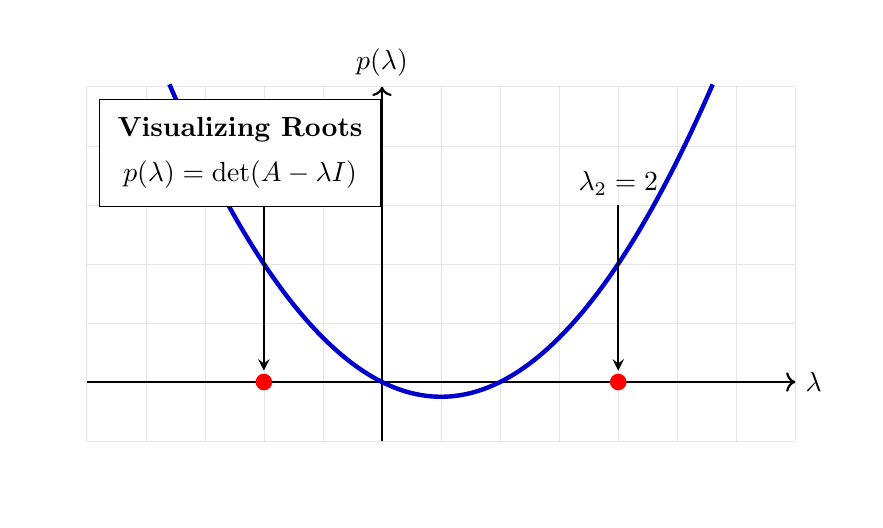
\begin{tikzpicture}[scale=1.5]
    % Background grid
    \fill[white] (-3,-1) rectangle (4,3);
    \draw[step=0.5cm, gray!20, very thin] (-2.5,-0.5) grid (3.5,2.5);
    
    % Axes
    \draw[thick, ->] (-2.5,0) -- (3.5,0) node[right, text=black] {$\lambda$};
    \draw[thick, ->] (0,-0.5) -- (0,2.5) node[above, text=black] {$p(\lambda)$};
    
    % Curve for lambda^2 - 4\lambda - 45 (scaled and shifted for visual representation of roots at -1 and 2)
    % Let's plot a generic characteristic polynomial p(\lambda) = (\lambda + 1)(\lambda - 2) = \lambda^2 - \lambda - 2
    \draw[ultra thick, blue!80!black, domain=-1.8:2.8, samples=100] plot (\x, {0.5*(\x*\x - \x - 2) + 1});
    
    % Roots (Eigenvalues)
    \fill[red] (-1, 0) circle (2pt);
    \fill[red] (2, 0) circle (2pt);
    
    % Callouts
    \draw[->, >=stealth, shorten >=2pt, thick] (-1, 1.5) -- (-1,0.05);
    \node[above, text=black] at (-1, 1.5) {$\displaystyle \lambda_1 = -1$};
    
    \draw[->, >=stealth, shorten >=2pt, thick] (2, 1.5) -- (2,0.05);
    \node[above, text=black] at (2, 1.5) {$\displaystyle \lambda_2 = 2$};
    
    % Legend
    \matrix [matrix of nodes, draw=black, fill=white, anchor=north west] at (-2.4, 2.4) {
        \node[text=black] {\textbf{Visualizing Roots}}; \\
        \node[text=black] {$\displaystyle p(\lambda) = \det(A - \lambda I)$}; \\
    };
\end{tikzpicture}

\newpage
\section{Conceptual Synthesis and The "Big Picture"}

\subsection{Thematic Connections}
The central theme of the characteristic equation is \textbf{invariance}. In calculus, we look for functions that are invariant under differentiation (e.g., $f(x) = e^x$, where $\frac{d}{dx}e^x = e^x$). In linear algebra, eigenvalues represent the exact same concept: vectors that are invariant in direction under a matrix transformation ($Ax = \lambda x$). The characteristic equation is the algebraic tool used to hunt down these invariant properties.

\subsection{Forward and Backward Links}
\textbf{Backward Links:} This topic relies heavily on the theory of determinants and the Invertible Matrix Theorem. The realization that a non-trivial null space requires a determinant of zero is the logical bedrock of the characteristic equation.

\textbf{Forward Links:} Mastering the characteristic equation is the absolute prerequisite for \textbf{Diagonalization}. If a matrix has enough linearly independent eigenvectors, it can be factored into $A = PDP^{-1}$, where $D$ is a diagonal matrix of eigenvalues. This makes computing massive matrix powers ($A^k = PD^kP^{-1}$) computationally trivial, which is the foundation for solving systems of linear differential equations and analyzing Markov chains.

\section{Abstract Real-World Modeling (AI, ML, \& Quant Finance)}

\subsection{Concrete Scenarios}
\begin{enumerate}
    \item \textbf{Principal Component Analysis (PCA) in Machine Learning:} In high-dimensional datasets (like images or genomic data), ML engineers use PCA to reduce dimensionality. They compute the covariance matrix of the data and find its eigenvalues via the characteristic equation. The largest eigenvalues correspond to the "principal components" that capture the most variance in the data.
    \item \textbf{Markov Chains in Quantitative Finance:} Quants model stock market regimes (e.g., Bull, Bear, Stagnant) using transition matrices. The long-term, steady-state probability of being in any given market regime is found by solving for the eigenvector corresponding to the eigenvalue $\lambda = 1$.
\end{enumerate}

\subsection{Model Problem Setup: PCA Covariance Modeling}
Let $X \in \R^{n \times p}$ be a centered data matrix representing $n$ financial assets over $p$ time periods. The sample covariance matrix is defined as:
\[ \Sigma = \frac{1}{n-1} X^T X \]
$\Sigma$ is a $p \times p$ symmetric, positive semi-definite matrix. To find the orthogonal axes of maximum variance (the principal components), we must solve the eigenvalue problem:
\[ \Sigma v = \lambda v \]
This requires finding the roots of the characteristic polynomial:
\[ \det(\Sigma - \lambda I) = 0 \]
Because $\Sigma$ is symmetric, the Spectral Theorem guarantees that all eigenvalues $\lambda_1 \geq \lambda_2 \geq \dots \geq \lambda_p \geq 0$ are real. The total variance of the financial system is the trace of $\Sigma$, which equals $\sum \lambda_i$. An algorithmic trading model might project the original data onto the eigenvectors corresponding to the top 3 eigenvalues, effectively filtering out market noise and reducing the state space from $p$ dimensions to 3, allowing for faster, more robust statistical arbitrage calculations.

\newpage
\section{Common Variations and Untested Concepts}

The provided homework focused exclusively on real eigenvalues and basic multiplicities. However, standard curriculums heavily test two additional variations:

\subsection{Variation 1: Complex Eigenvalues}
Not all matrices have real eigenvalues. Matrices that represent rotations in space will have complex eigenvalues, because no real vector maintains its direction during a pure rotation.
\textbf{Example:} Find the eigenvalues of the $90^\circ$ rotation matrix $A = \begin{bmatrix} 0 & -1 \\ 1 & 0 \end{bmatrix}$.
\begin{align*}
    \det(A - \lambda I) &= \det \begin{bmatrix} -\lambda & -1 \\ 1 & -\lambda \end{bmatrix} \\
    &= (-\lambda)(-\lambda) - (-1)(1) \\
    &= \lambda^2 + 1 = 0
\end{align*}
The roots are $\lambda = \pm i$. Complex eigenvalues always occur in conjugate pairs for real matrices and indicate oscillatory or rotational dynamics.

\subsection{Variation 2: Defective Matrices (Algebraic vs. Geometric Multiplicity)}
The \textit{algebraic multiplicity} is how many times $\lambda$ appears as a root of the characteristic polynomial. The \textit{geometric multiplicity} is the dimension of the eigenspace (the number of linearly independent eigenvectors for that $\lambda$). 
\textbf{Crucial Theorem:} Geometric Multiplicity $\leq$ Algebraic Multiplicity.
If the geometric multiplicity is strictly less than the algebraic multiplicity, the matrix is called \textbf{defective} and cannot be diagonalized.

\textbf{Example:} $A = \begin{bmatrix} 2 & 1 \\ 0 & 2 \end{bmatrix}$. 
The characteristic polynomial is $(2 - \lambda)^2 = 0$, so $\lambda = 2$ has an algebraic multiplicity of 2. 
However, solving $(A - 2I)x = 0$ yields:
\[ \begin{bmatrix} 0 & 1 \\ 0 & 0 \end{bmatrix} \begin{bmatrix} x_1 \\ x_2 \end{bmatrix} = \begin{bmatrix} 0 \\ 0 \end{bmatrix} \implies x_2 = 0 \]
The eigenvectors are of the form $x = \begin{bmatrix} x_1 \\ 0 \end{bmatrix} = x_1 \begin{bmatrix} 1 \\ 0 \end{bmatrix}$. There is only 1 basis vector, so the geometric multiplicity is 1. The matrix is defective.

\newpage
\section{Advanced Diagnostic Testing: "Find the Flaw"}

Below are 5 problems with fully worked solutions. Each solution contains a single, subtle, yet critical flaw. Your task as the grader is to identify the error, explain why it is wrong in one sentence, and provide the correct final solution.

\subsection{Problem 1}
\textbf{Question:} Find the characteristic polynomial of $A = \begin{bmatrix} 4 & 2 \\ 3 & 1 \end{bmatrix}$.
\textbf{Flawed Solution:}
Using the $2 \times 2$ shortcut formula, the characteristic polynomial is $\lambda^2 + \text{tr}(A)\lambda + \det(A) = 0$.
The trace is $4 + 1 = 5$. The determinant is $(4)(1) - (2)(3) = 4 - 6 = -2$.
Therefore, the polynomial is $\lambda^2 + 5\lambda - 2 = 0$.

\subsection{Problem 2}
\textbf{Question:} Find the eigenvalues of $A = \begin{bmatrix} 2 & 0 & 0 \\ 1 & 3 & 0 \\ 4 & 5 & -1 \end{bmatrix}$.
\textbf{Flawed Solution:}
To find the characteristic polynomial, we multiply the diagonal entries because it is a triangular matrix:
$p(\lambda) = (2)(3)(-1) = -6$.
Setting $-6 - \lambda = 0$, we get $\lambda = -6$.

\subsection{Problem 3}
\textbf{Question:} Let $A = \begin{bmatrix} 1 & 4 \\ 2 & 3 \end{bmatrix}$. Find the eigenvalues of $A^2$.
\textbf{Flawed Solution:}
First, we find the eigenvalues of $A$. $\text{tr}(A) = 4$, $\det(A) = -5$.
$p(\lambda) = \lambda^2 - 4\lambda - 5 = (\lambda - 5)(\lambda + 1) = 0$. The eigenvalues of $A$ are $5$ and $-1$.
To find the eigenvalues of $A^2$, we simply multiply the eigenvalues of $A$ by 2.
Thus, the eigenvalues of $A^2$ are $10$ and $-2$.

\subsection{Problem 4}
\textbf{Question:} Find the characteristic polynomial of $A = \begin{bmatrix} 1 & 2 & 3 \\ 0 & 4 & 5 \\ 0 & 0 & 6 \end{bmatrix}$.
\textbf{Flawed Solution:}
We set up $\det(A - \lambda I) = 0$.
\[ \det \begin{bmatrix} 1 - \lambda & 2 & 3 \\ 0 & 4 & 5 \\ 0 & 0 & 6 \end{bmatrix} = 0 \]
Expanding along the first column:
$(1 - \lambda) \left[ (4)(6) - (5)(0) \right] = (1 - \lambda)(24) = 24 - 24\lambda$.
The characteristic polynomial is $24 - 24\lambda$.

\subsection{Problem 5}
\textbf{Question:} A $3 \times 3$ matrix $A$ has a characteristic polynomial $p(\lambda) = -\lambda^3 + 6\lambda^2 - 9\lambda$. Determine if $A$ is invertible.
\textbf{Flawed Solution:}
We factor the polynomial: $-\lambda(\lambda^2 - 6\lambda + 9) = -\lambda(\lambda - 3)^2$.
The eigenvalues are $\lambda = 0$ and $\lambda = 3$.
Since the eigenvalue $\lambda = 3$ has an algebraic multiplicity of 2, the matrix has multiple non-zero eigenvalues, which means its determinant is non-zero. Therefore, $A$ is invertible.

\vspace{1cm}
\hrule
\vspace{0.5cm}
\textbf{Grader Answer Key (For your reference):}
\begin{itemize}
    \item \textbf{Flaw 1:} The shortcut formula is $\lambda^2 - \text{tr}(A)\lambda + \det(A)$, not $+ \text{tr}(A)\lambda$. Correct polynomial: $\lambda^2 - 5\lambda - 2$.
    \item \textbf{Flaw 2:} The student multiplied the matrix entries directly instead of the diagonal entries of $(A - \lambda I)$. Correct eigenvalues are the diagonal entries themselves: $2, 3, -1$.
    \item \textbf{Flaw 3:} If $\lambda$ is an eigenvalue of $A$, then $\lambda^2$ is an eigenvalue of $A^2$, not $2\lambda$. Correct eigenvalues are $25$ and $1$.
    \item \textbf{Flaw 4:} The student forgot to subtract $\lambda$ from the other diagonal entries $4$ and $6$ before expanding. Correct polynomial: $(1-\lambda)(4-\lambda)(6-\lambda)$.
    \item \textbf{Flaw 5:} The student ignored the eigenvalue $\lambda = 0$; if $0$ is an eigenvalue, the determinant is $0$, making the matrix non-invertible.
\end{itemize}

\end{document}